%%%%%%%%%%%%%%%%%%%%%%%%%%%%%%%%%%%%%%%%
%% MCM/ICM LaTeX Template %%
%% 2025 MCM/ICM %%
%%%%%%%%%%%%%%%%%%%%%%%%%%%%%%%%%%%%%%%%

% Format
\documentclass[12pt]{article}
\usepackage{geometry}
\geometry{left=1in, right=0.75in, top=1in, bottom=1in}

\newcommand{\Problem}{F}
\newcommand{\Team}{2500434}

\usepackage{newtxtext}
\usepackage{amsmath,amssymb,amsthm}
\usepackage{newtxmath}
\usepackage[pdftex]{graphicx}
\usepackage{xcolor}
\usepackage{fancyhdr}
\usepackage{enumitem}
\usepackage{titlesec}
\usepackage{tocloft}
\usepackage{lastpage}

% Page Settings
\pagestyle{fancy}
\lhead{Team \# \Team}
\rhead{Page \thepage\ of \pageref{LastPage}}

% Mathematical env.
\newtheorem{theorem}{Theorem}
\newtheorem{corollary}[theorem]{Corollary}
\newtheorem{lemma}[theorem]{Lemma}
\newtheorem{definition}{Definition}

% Format of table of contents
\renewcommand{\cftsecleader}{\cftdotfill{\cftdotsep}}
\renewcommand{\contentsname}{\begin{center} INDEX \end{center}}

% Format of subsection and subsubsection
\titleformat{\section}{\bfseries\centering\Large}{\thesection}{1em}{}
\titleformat{\subsection}{\bfseries\raggedright}{\thesubsection}{1em}{}{}
\titleformat{\subsubsection}{\bfseries}{\hspace*{2em}\thesubsubsection}{1em}{}{}

% CoverPage Design
\begin{document}
\graphicspath{{.}}  % Place the graphic file in the same directory as the main document
\DeclareGraphicsExtensions{.pdf, .jpg, .tif, .png}
\thispagestyle{empty}
\vspace*{-16ex}
\centerline{
\begin{tabular}{*3{c}}
	\parbox[t]{0.3\linewidth}{\begin{center}\textbf{Problem Chosen}\\ \Large \textcolor{red}{\Problem}\end{center}}
	& \parbox[t]{0.3\linewidth}{\begin{center}\textbf{2025\\ MCM/ICM\\ Summary Sheet}\end{center}}
	& \parbox[t]{0.3\linewidth}{\begin{center}\textbf{Team Control Number}\\ \Large \textcolor{red}{\Team}\end{center}}	\\
	\hline
\end{tabular}}

% TODO: Summary
% 1. 12-point Times New Roman font ;
% 2. pdf naming format: 2500434.pdf ;
% 3. No name of school, advisor, or team members .
\begin{center}
Hello Summary!
\end{center}

\newpage
\tableofcontents
\newpage

\section{Introduction}\label{sec:introduction} %1
	\subsection{Background}\label{subsec:background} %1.1
		In the digital age, the speed and scale of global connectivity have reached unprecedented heights.
		However, with technological advancements, \( \textbf{cybercrime} \) has also become increasingly complex and diverse.
		These crimes pose significant threats and challenges to personal privacy, corporate assets, national security, and social stability.
		The transnational and covert nature of cybercrime makes it difficult to address effectively.
		Attackers often exploit legal differences and technical vulnerabilities across countries to evade accountability.
		Additionally, many businesses and institutions, concerned about their reputation and commercial interests,
		often choose \( \textbf{not to publicly report} \) cyberattacks, opting instead to pay ransoms or handle incidents privately.
		This further exacerbates the hidden nature of cybercrime.
		Developed countries, with their highly digitized economic and social structures, are often prime targets for cybercrime, while
		developing countries face their own unique challenges.

		To address this global challenge, countries have introduced national cybersecurity \( \textbf{policies} \)
		aimed at enhancing their defensive capabilities through legal, technical, and organizational cooperation.
		The \( \textbf{effectiveness} \) of these policies varies significantly across nations, and these differences may be closely related to factors
		such as policy design, enforcement, technological infrastructure, education levels, economic development, and internet penetration rates.

		In this context, understanding which factors make certain countries' cybersecurity policies more effective has become a critical issue.
		By analyzing the global distribution of cybercrime, national cybersecurity policies, and their outcomes,
		we can identify which policies and laws are particularly effective in preventing, prosecuting, and mitigating cybercrime.
		This data-driven analysis not only helps countries improve their cybersecurity policies
		but also provides valuable insights for global cybersecurity cooperation.
	\subsection{Restatement of the problem}\label{subsec:restatement-of-the-problem} %1.2
		We are required to identify patterns that can inform the data-driven development and refinement of national cybersecurity policies and laws,
		which focused on those that have demonstrated effectiveness.
		Our goal is to develop a theory explaining what constitutes a strong national cybersecurity policy and then support it with a data-driven analysis.

		Several key aspects are listed below:
		\begin{itemize}
			\item Patterns in cybercrime distributed worldwide.
			\item Assessment to effectiveness of National Cybersecurity Policies.
			\item Correlation between national demographics and our distribution analysis.
		\end{itemize}
	\subsection{Analysis of problems}\label{subsec:analysis-of-problems} %1.3
		We have divided each problem into several different steps:
		\subsubsection[]{Cybercrime distribution across the world} %1.3.1
			\begin{itemize}
				\item Analyze the JSON files published on VCDB (the VERIS community database).
				\item Use the Global Cybersecurity Index (GCI) as the primary indicator to assess countries with disproportionately high levels of cybercrime.
				\item Group countries based on their implementation of similar policies over a period of time, and
					visually represent the distribution of cybercrime in each group using a 3D heatmap.
			\end{itemize}
		\subsubsection[]{Effective policy or law analytical approach} %1.3.2
			\begin{itemize}
				\item TODO % TODO: fill the blank
			\end{itemize}
		\subsubsection[]{National demographics correlation} %1.3.3
			\begin{itemize}
				\item TODO % TODO: fill the blank
			\end{itemize}
	
\section{Symbol and Assumptions}\label{sec:symbol-and-assumptions} %2
	\subsection{Symbol Description}\label{subsec:symbol-description} %2.1
		TODO % TODO: list all symbols
	\subsection{Assumption}\label{subsec:assumption} %2.2
		\begin{itemize}
			\item Countries with a population below \( "TODO" \) are excluded from the consideration of cybercrime distribution because
				a small change of number could bring a significant difference to statistical analysis.
			\item In the statistical analysis of the global distribution of cybercrime,
				factors such as national population growth, internet access, wealth levels, and education levels
				are assumed to have no significant impact on the quantitative distribution of cybercrime incidents.
				This study hypothesizes that the distribution of cybercrime can be more intuitively understood by focusing solely on the number of incidents,
				independent of these socio-economic variables.
				This assumption is based on all available data recorded since the inception of cybercrime statistics,
				aiming to isolate the distribution patterns of cybercrime from other potential influencing factors.
		\end{itemize}

\section{The establishment and solution of problem 1 model}\label{sec:the-establishment-and-solution-of-problem-1-model} %3
	Despite the continuous evolution of national cybercrime since the inception of data collection,
	along with changes in policies, legal frameworks, and population demographics,
	we can create a global cybercrime hotspot map by leveraging crime data recorded by VERIS over the years.
	This not only facilitates the analysis of cybercrime volumes by country
	but also allows for fitting the data against policy and population variables to assess their influence on cybercrime trends.
	\subsection{Cybercrime distribution across the globe}\label{subsec:Building-the-hotspot-map} %3.1
		We made use of a world-wide map to represent all cybercrime occurred around the world.
		In the map, the color filled in each country represents the total number of cybercrime incidents recorded since the beginning of the statistics.
		The color gradient, ranging from dark blue to dark red, corresponds to eight severity levels (1 to 8).
		Countries marked in blue indicate a low frequency of cybercrime incidents, while those marked in red represent a high density of such incidents.
		For instance, the United States, where the VERIS concept was first proposed, has the highest number of recorded incidents (7,236),
		whereas many other countries have only 1 or 2 recorded incidents.
		To address this significant disparity in data distribution, we applied a logarithmic transformation to the data using the formula
		\[ y=\log(1+x) \].
		This transformation was implemented using the function
		\[ np.log1p() \]
		in Python to ensure computational precision and stability, particularly for small values.
		The final results are visualized in Figure 1.
		\begin{figure}[htbp]
			\centering
			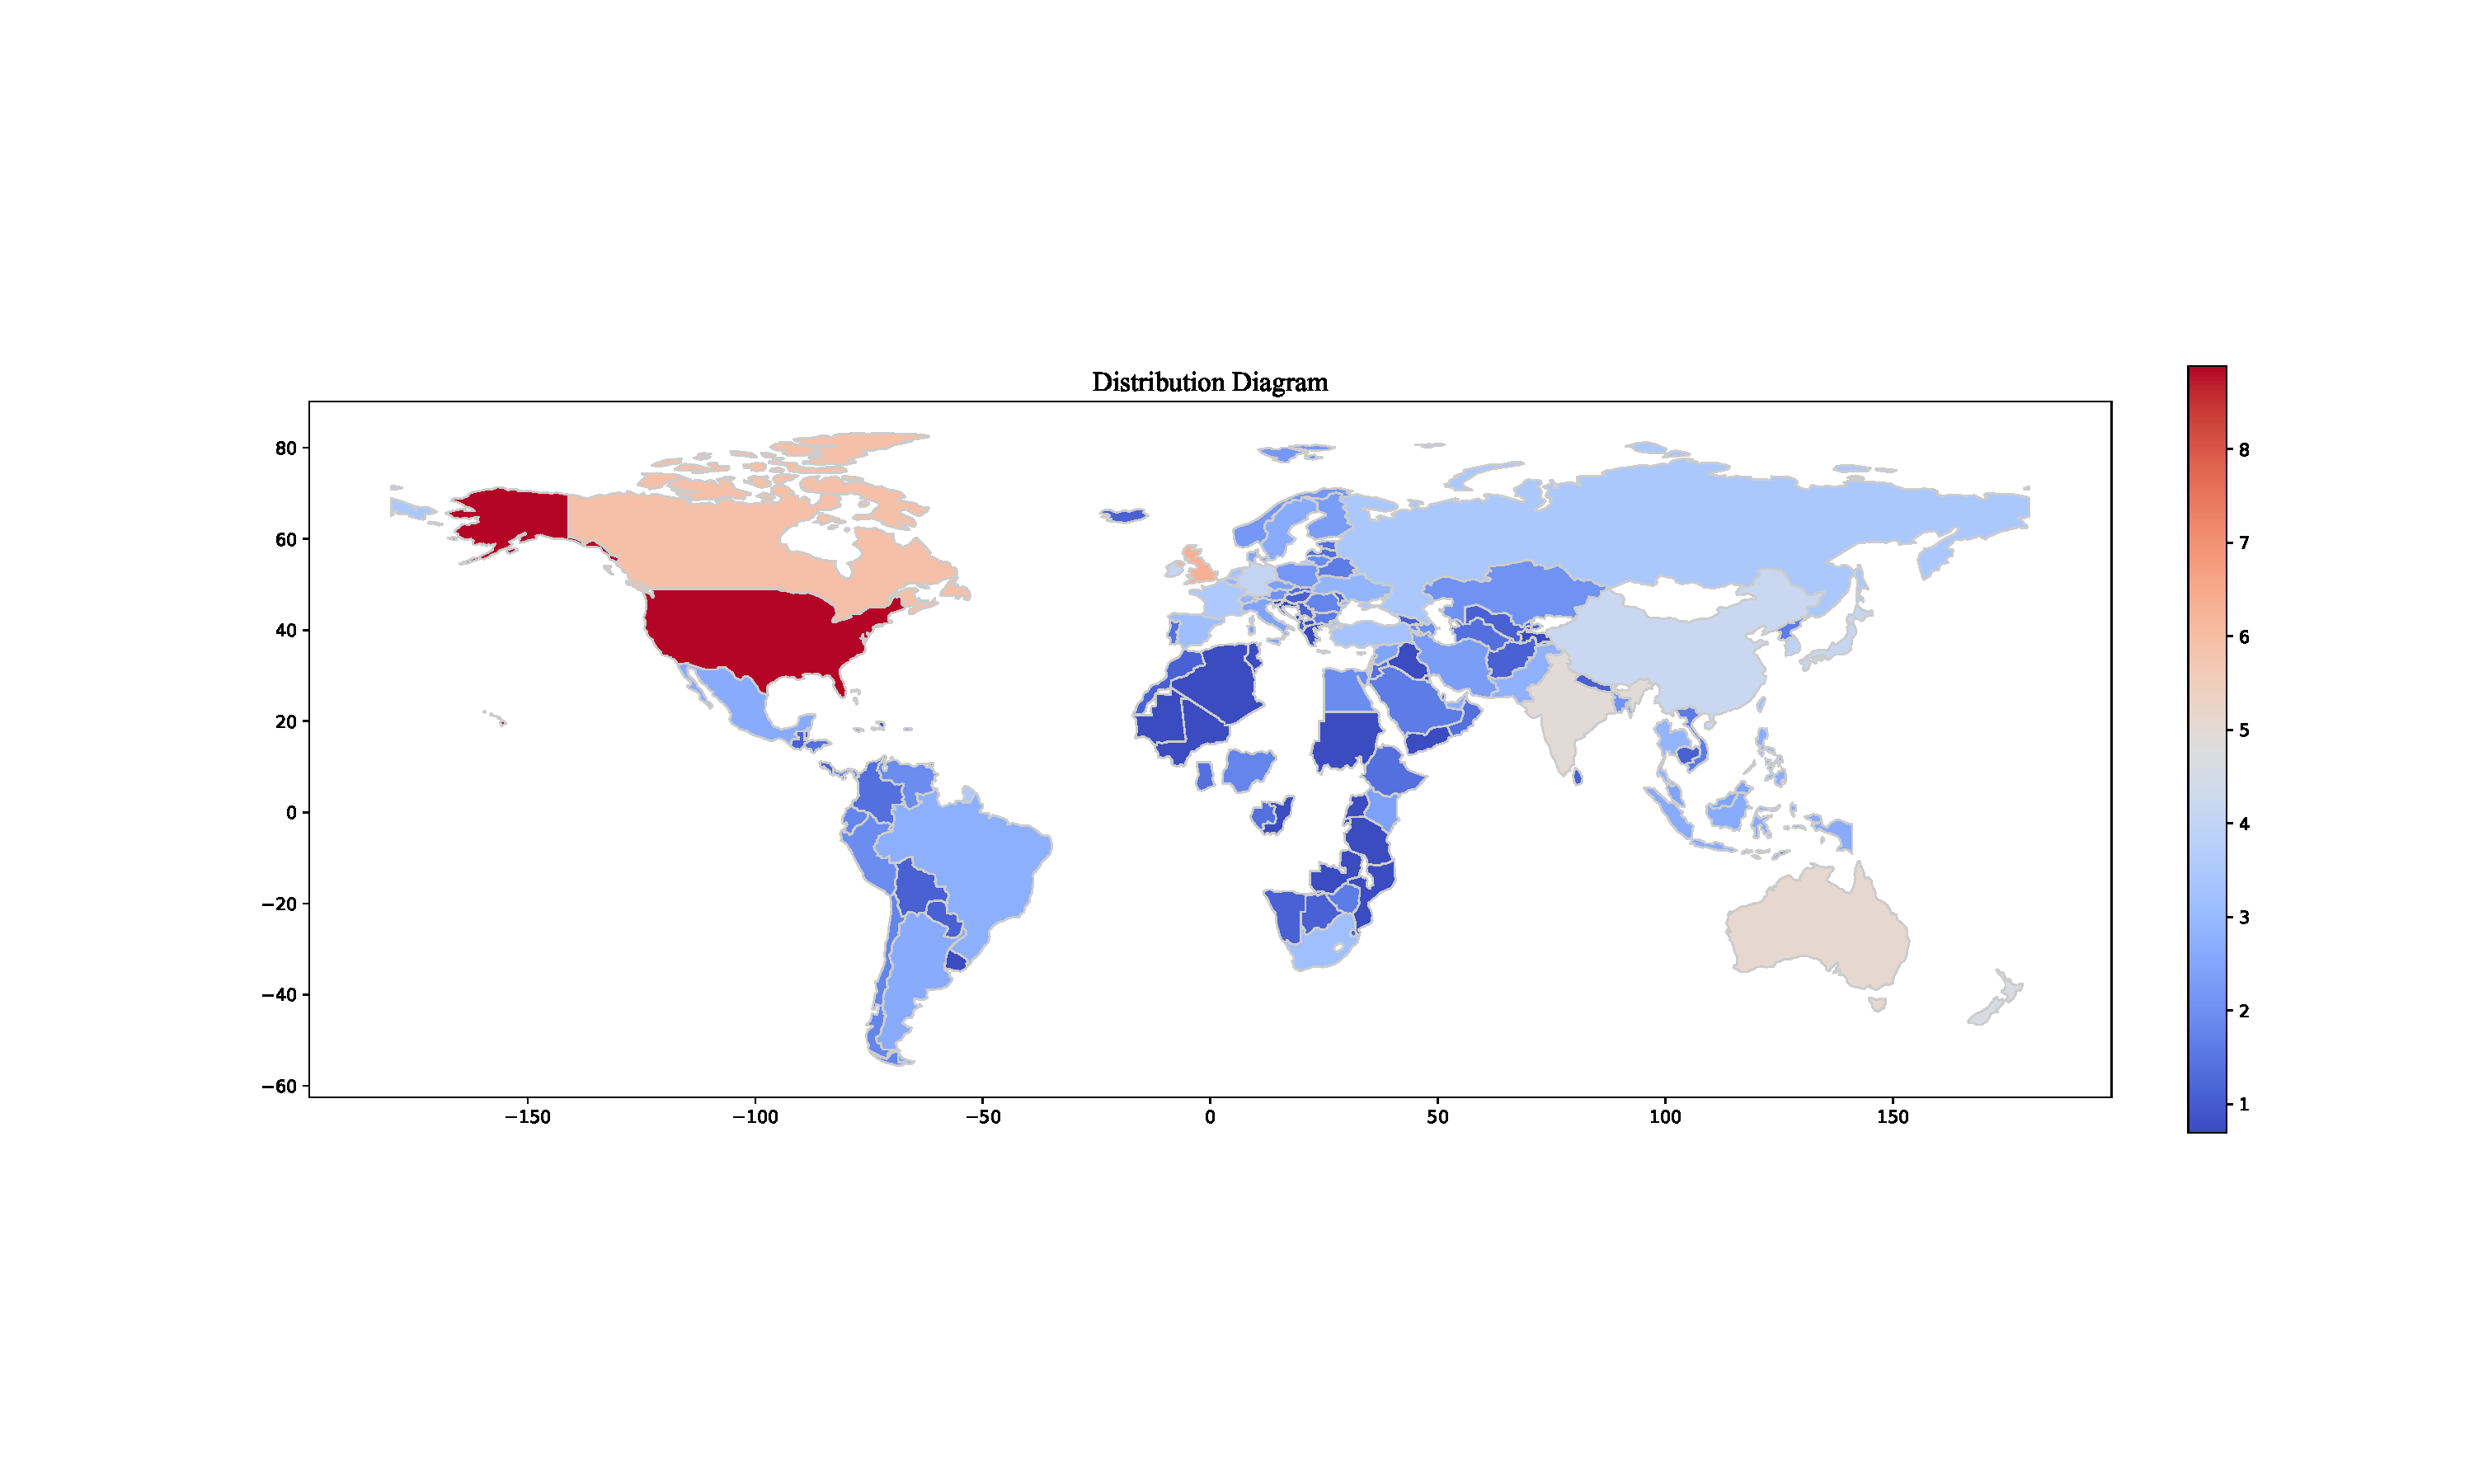
\includegraphics[width=1\textwidth]{./rsrc/Crime_distribution}
			\caption{Crime distribution}\label{fig:crime-distribution}
		\end{figure}
	\subsection{High-prevalence regions}\label{subsec:high-prevalence-regions} %3.2
	\subsection{Other Cybercrime Incidents}\label{subsec:other-cybercrime-incedents} % 3.3

		\begin{figure}[htbp]
			\centering
			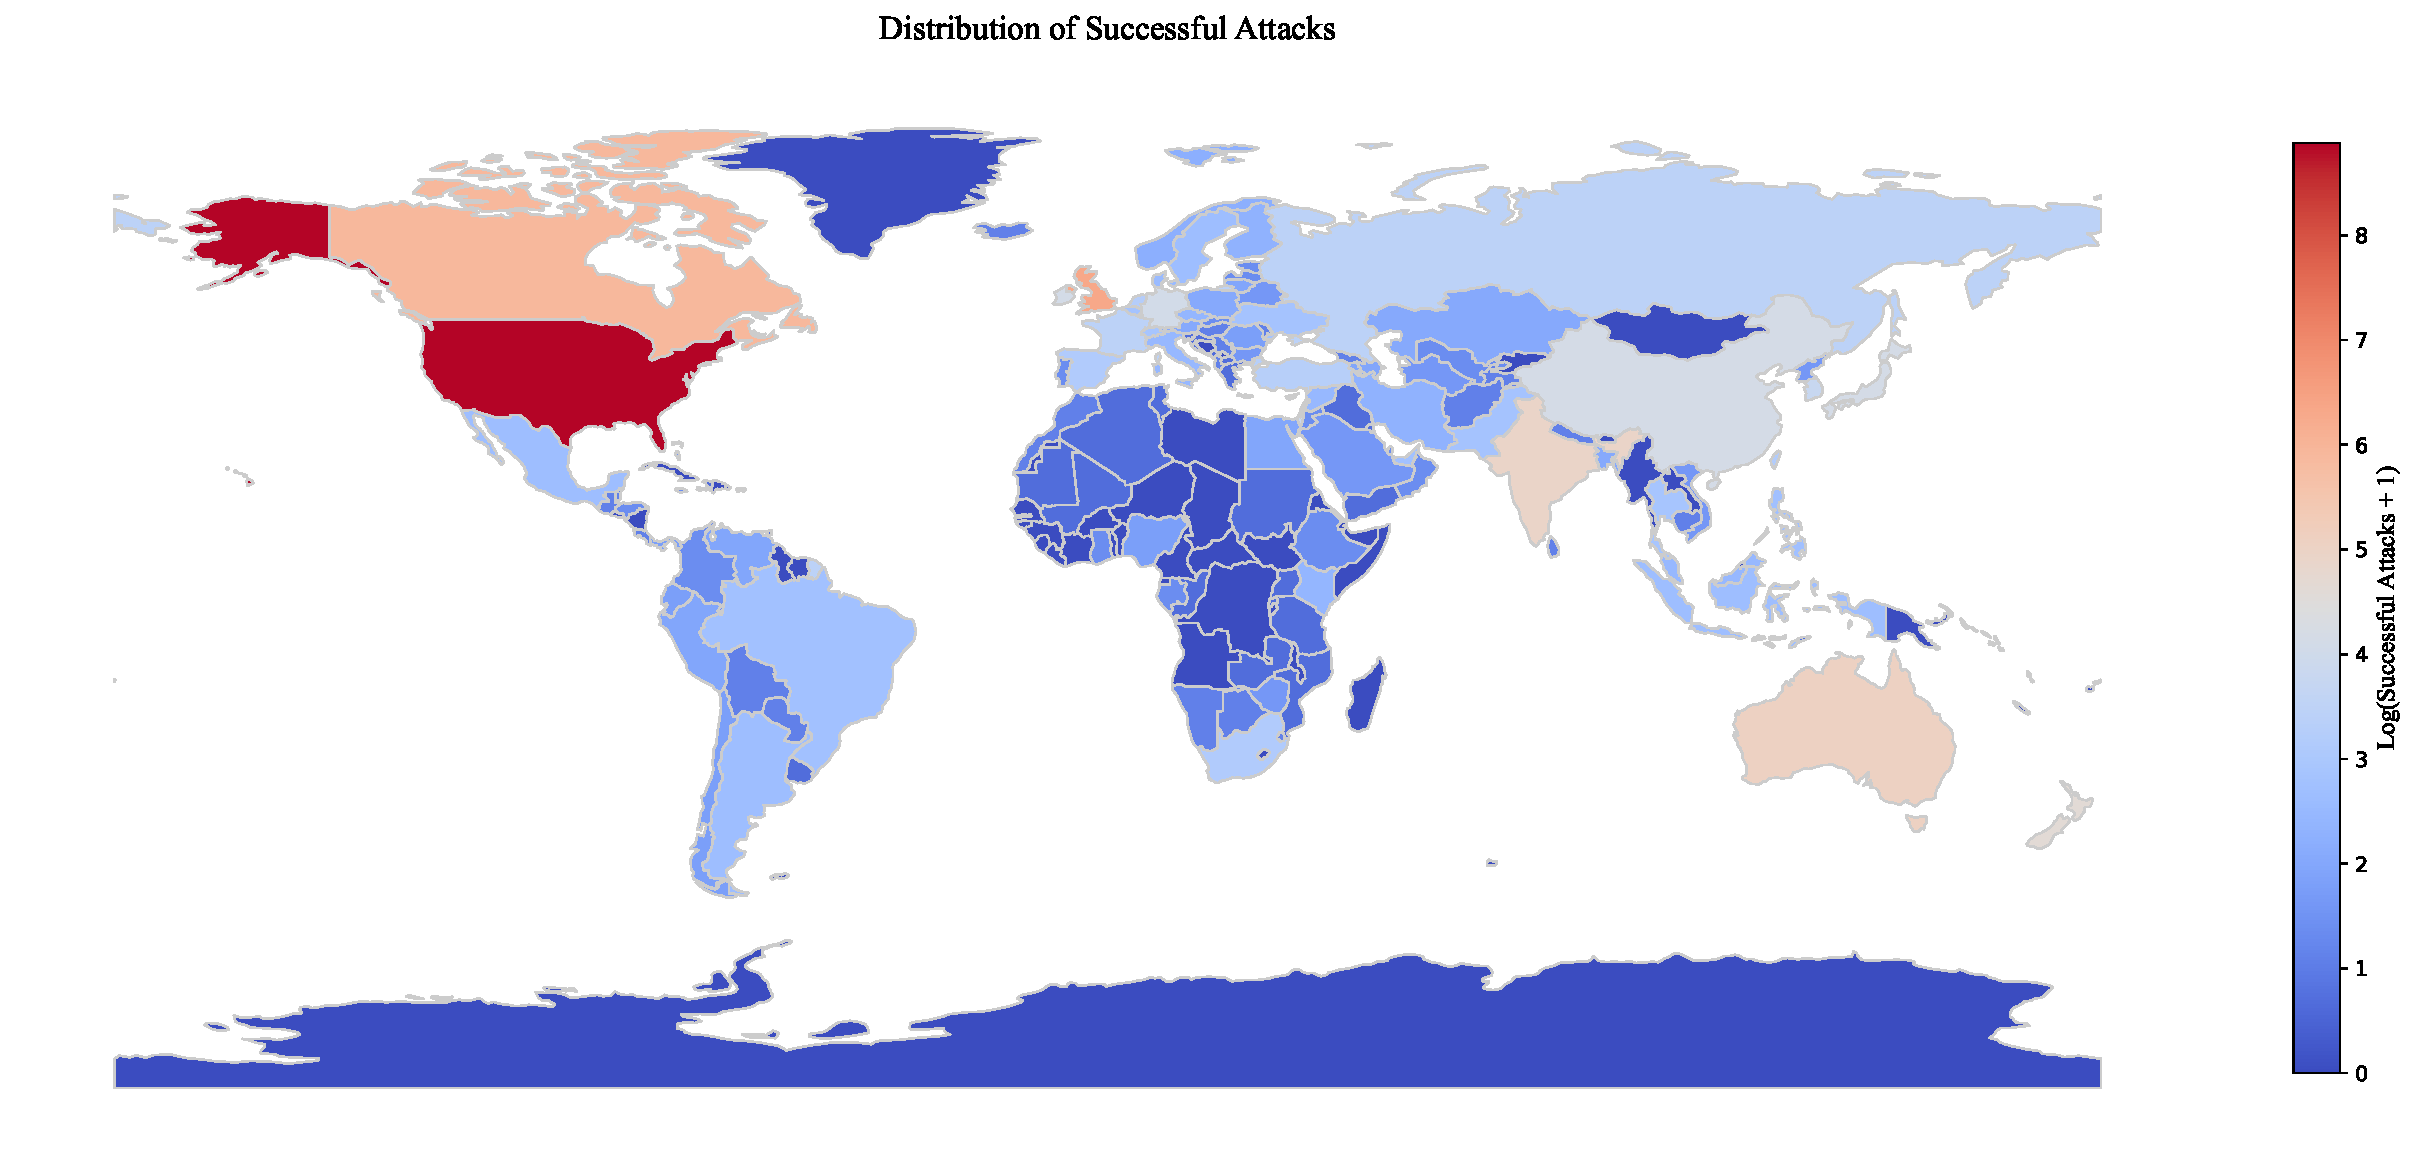
\includegraphics[width=1\textwidth]{./rsrc/Crime_Successful_distribution}
			\caption{Successful Cybercrime Incidents}\label{fig:successful-cybercrime-incidents}
		\end{figure}
		\begin{figure}[htbp]
			\centering
			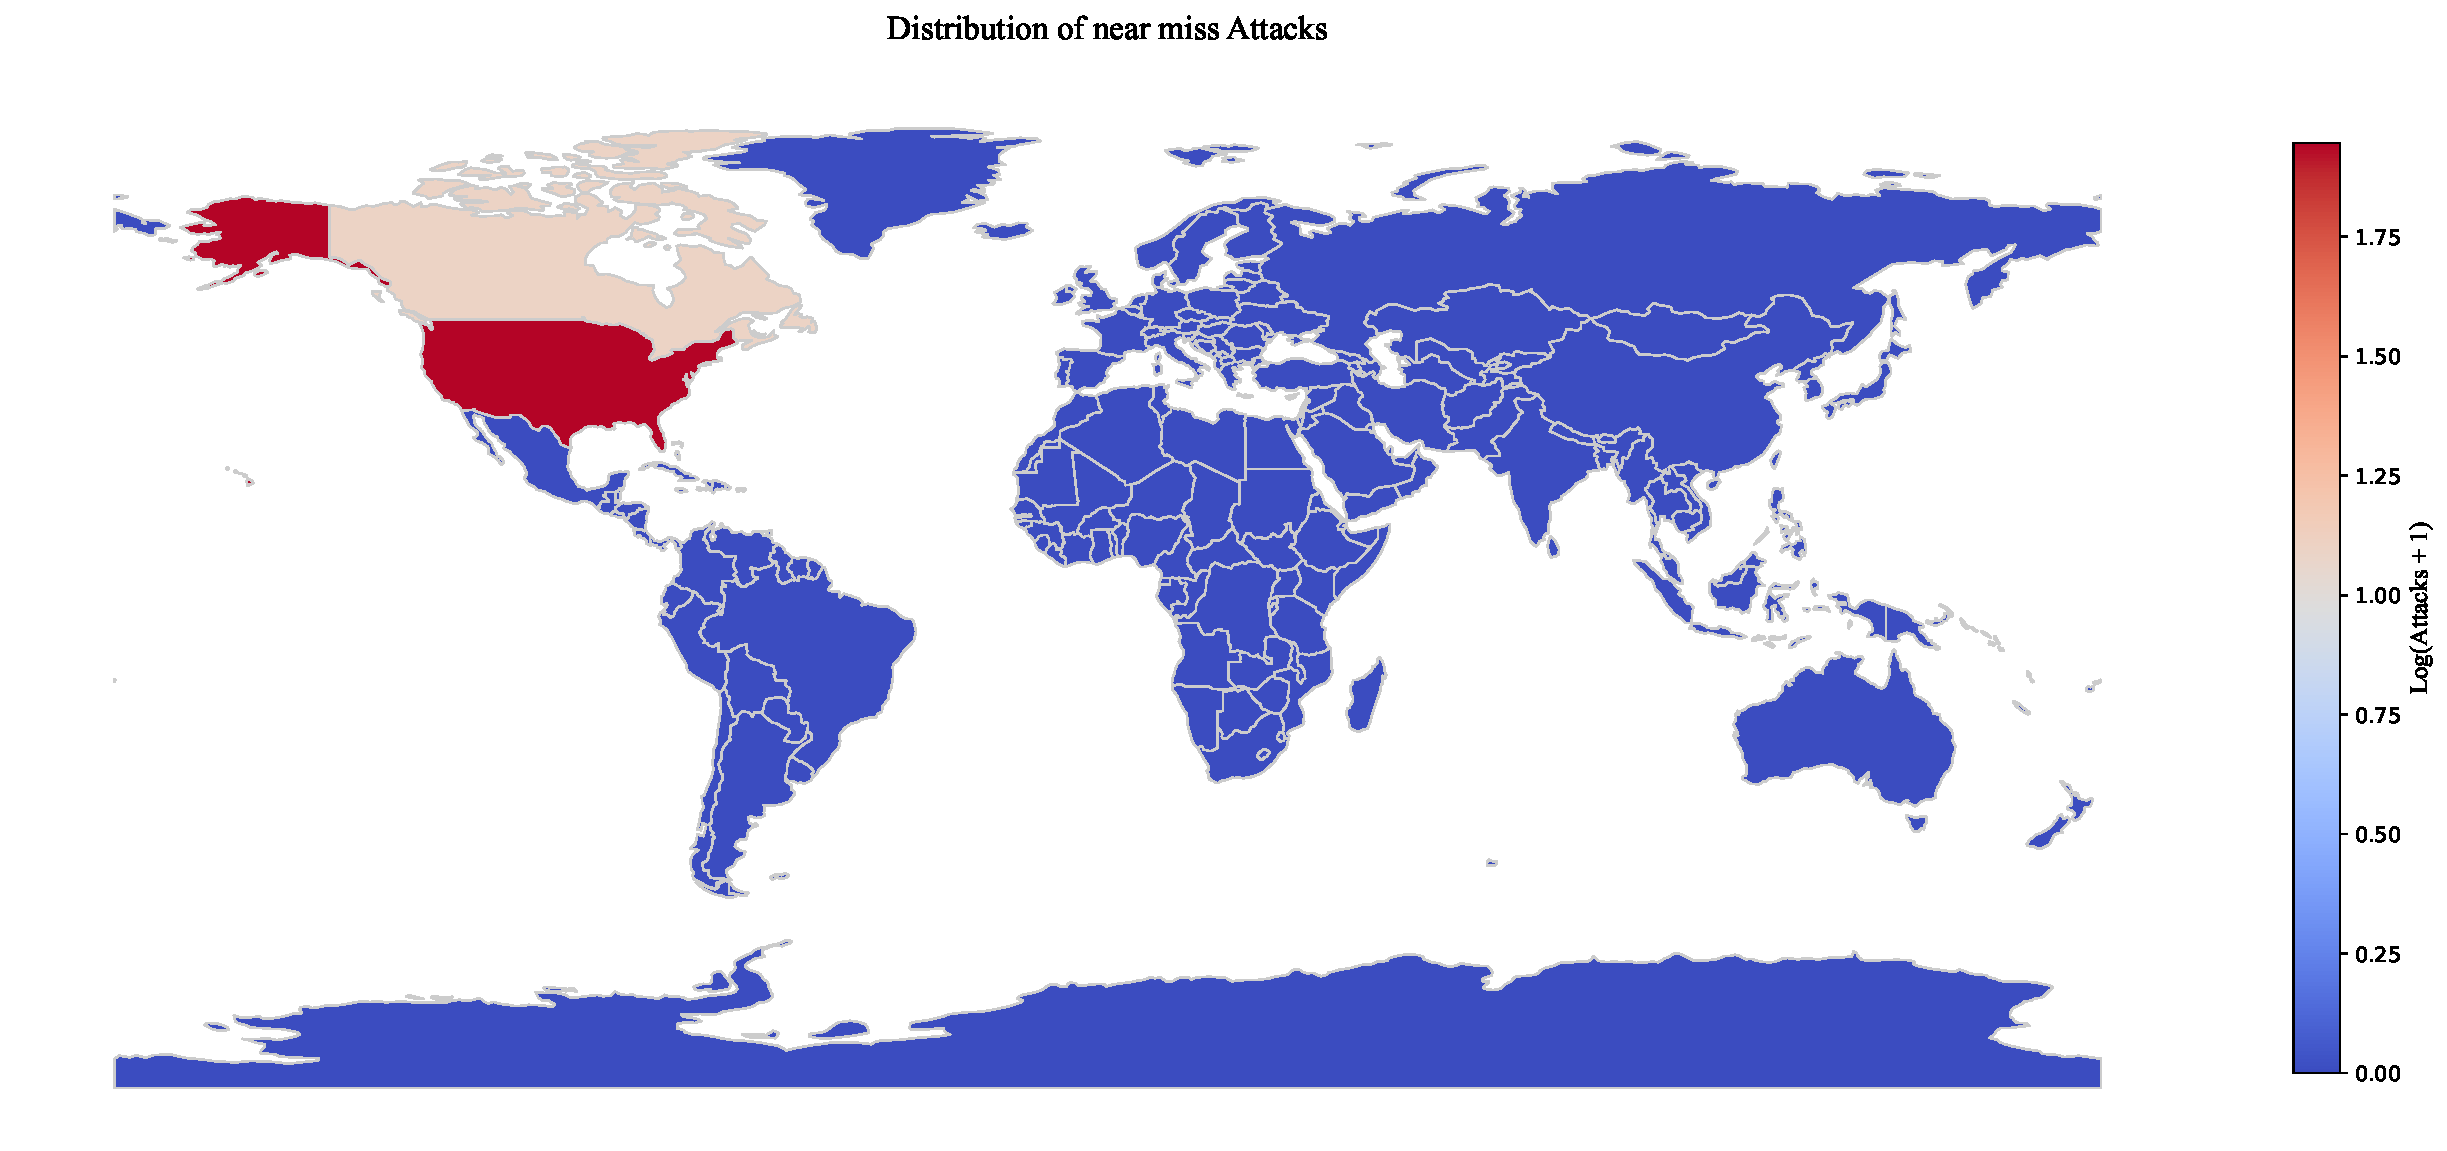
\includegraphics[width=1\textwidth]{./rsrc/Crime_NearMiss_distribution}
			\caption{Mitigated Cybercrime Attempts}\label{fig:mitigated-cybercrime-attempts}
		\end{figure}
		\begin{figure}[htbp]
			\centering
			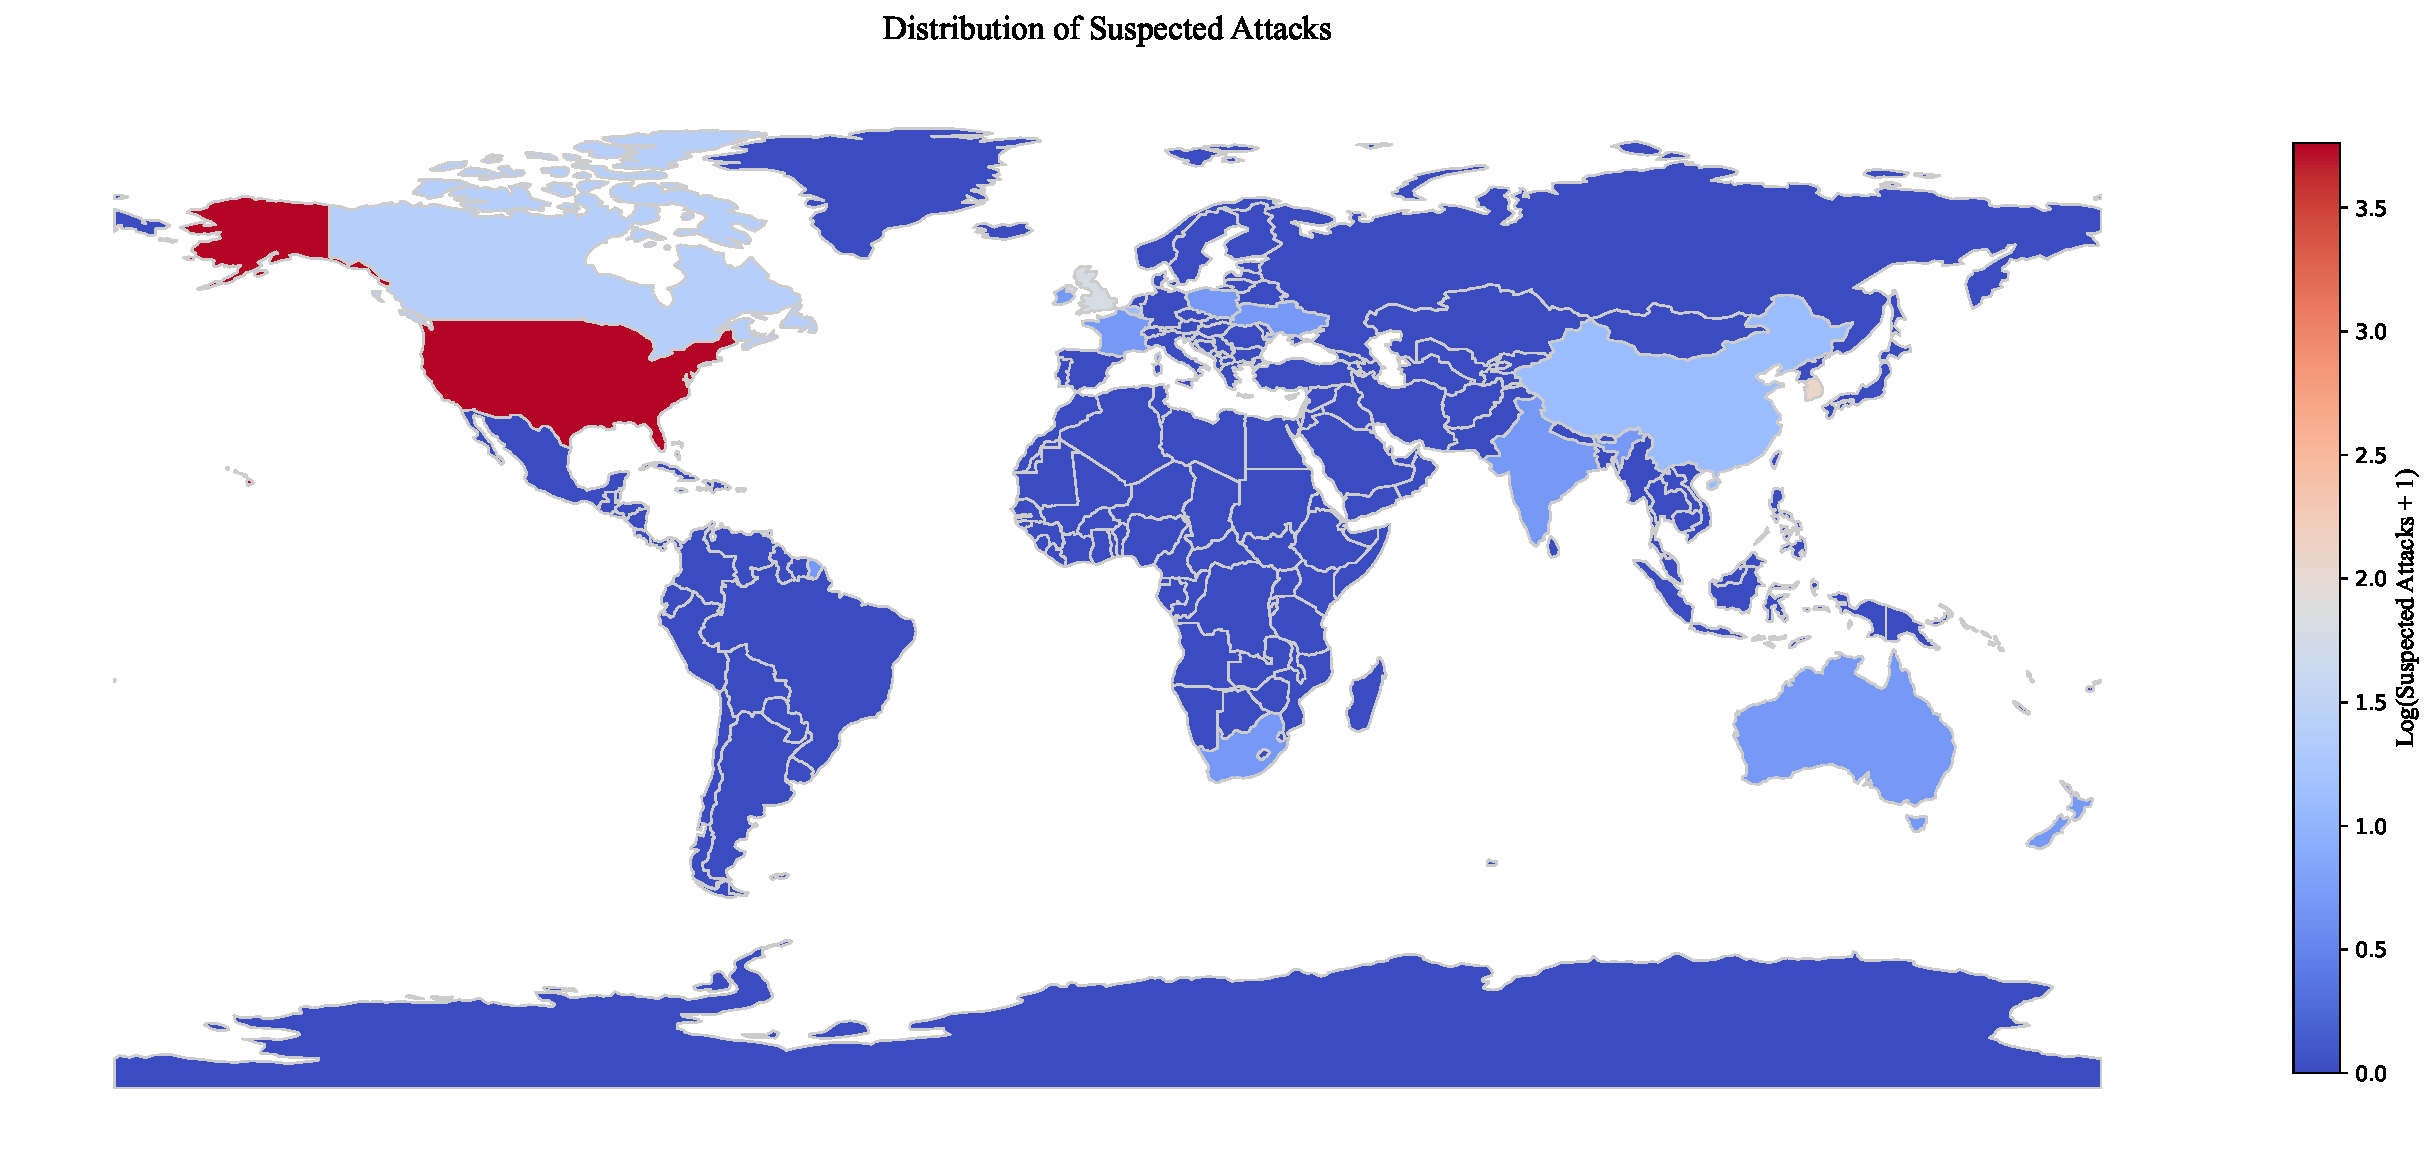
\includegraphics[width=1\textwidth]{./rsrc/Crime_Suspected_distribution}
			\caption{Reported Cybercrime Incidents}\label{fig:reported-cybercrime-incidents}
		\end{figure}

\section{The establishment and solution of problem 2 model}\label{sec:the-establishment-and-solution-of-problem-2-model} %4
	\subsection{Shit, bro*2}\label{subsec:shit-bro*2} %4.1
	
\section{The establishment and solution of problem 3 model}\label{sec:the-establishment-and-solution-of-problem-3-model} %5
	\subsection{Shit, bro*3}\label{subsec:shit-bro*3} %5.1
	
\section{Future expected data}\label{sec:future-expected-data} %6

\section{Advantages \& Disadvantages}\label{sec:advantages-&-disadvantages} %7

\section{References}\label{sec:references} %8

\section{Appendix}\label{sec:appendix} %9


\end{document}